%**************************************************
%			Improvements.tex
%**************************************************
\section{Improvements}
\frame
{
\frametitle{Weaknesses}
\tableofcontents[currentsection]
\addtocounter{framenumber}{-1}
}

\begin{frame}{Improvements}
Some improvements are:
\begin{itemize}
\item<2-> the NICE module
\item<3-> the FRESCO framework
\item<4-> algorithm for anomaly traffic detection
\end{itemize}
\end{frame}

\subsection{NICE module}
\begin{frame}{NICE module}
NICE is Intrusion Prevention System composed by two phases:
\begin{itemize}
\item<2-> NICE-A phase
\item<3-> Deep Packet Inspection phase
\end{itemize}
\end{frame}

\subsection{FRESCO framework}
\begin{frame}{FRESCO framework}
\begin{figure}
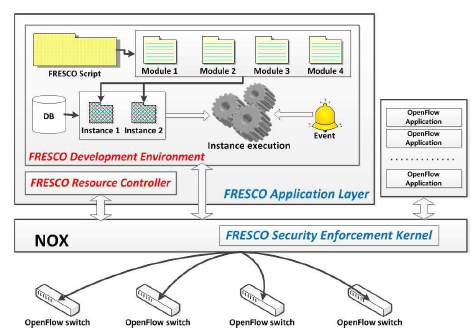
\includegraphics[scale=0.55]{Immagini/FrescoStructure.png}
\caption{FRESCO module}
\label{fig:FRESCO-module}
\end{figure}
\end{frame}

\subsection{Anomaly traffic detection}
\begin{frame}{Anomaly traffic detection}
Some algorithms to anomaly traffic detection are:
\begin{itemize}
\item<2-> Threshold Random Walk with Credit Based (TRW-CB)
\item<3-> Rate Limiting (RL)
\item<4-> Maximum Entropy Detector (MED)
\end{itemize}
\end{frame}